\documentclass[a4paper, 10pt, final, garamond]{book}
\usepackage{cours-preambule}
\graphicspath{{./figures/}}

\makeatletter
\renewcommand{\@chapapp}{Contr\^ole de connaissances}
\makeatother

% \toggletrue{student}
% \toggletrue{corrige}
\renewcommand{\mycol}{black}
% \renewcommand{\mycol}{gray}

\begin{document}
\setcounter{chapter}{23}

\settype{enon}
\settype{solu}

\chapter{Diagrammes $E-\pH$\ifstudent{~(13')}}

\begin{enumerate}[label=\sqenumi]
	\nitem{22}%
	\noindent
	\begin{minipage}[t]{.65\linewidth}
		On donne l'allure du diagramme du fer ci-contre. Les espèces à placer sont
		$\ce{Fe}_{\rm(s)}$, $\ce{{Fe}^2+_{\rm(aq)}}$, $\ce{{Fe}^3+_{\rm(aq)}}$,
		$\ce{{Fe(OH)_2}_{\rm(s)}}$ et $\ce{{Fe(OH)_3}_{\rm(s)}}$. On donne de plus~:
		\begin{itemize}
			\item $E_1^\circ(\ce{{Fe}^2+_{\rm(aq)}/Fe}) = \SI{-.44}{V}$~;
			      $E_2^\circ(\ce{{Fe}^3+_{\rm(aq)}/{Fe}^2+_{\rm(aq)}}) =
				      \SI{0.77}{V}$~;
			\item $\pk[s,2] = \pk[s](\ce{Fe(OH)_2}) = 15$ et $\pk[s,3] =
				      \pk[s](\ce{Fe(OH)_3}) = 38$~;
			\item Convention de tracé $c_t = \SI{0.01}{mol.L^{-1}}$.
		\end{itemize}
		\textbf{Remplir sans démonstration le diagramme $E-\pH$, déterminer la
			position des frontières verticales, puis les pentes des frontières
			inclinées}.
	\end{minipage}
	\hfill
	\begin{minipage}[t]{.32\linewidth}
		\vspace{-20pt}
		\begin{center}
			\sswitch{
				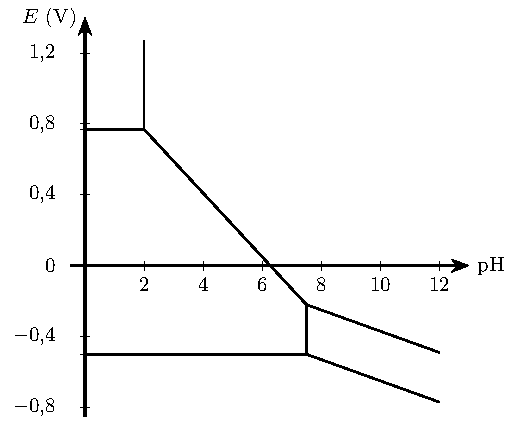
\includegraphics[width=\linewidth]{eph_fer-plain}
			}{
				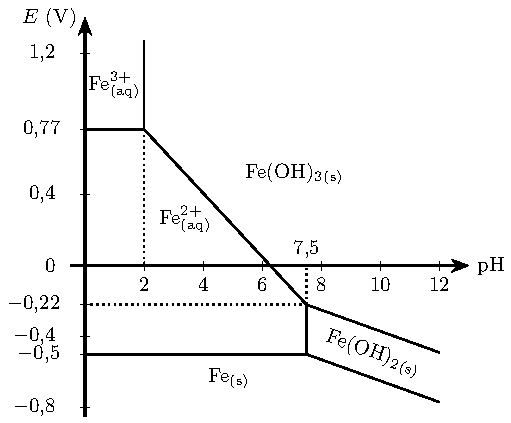
\includegraphics[width=\linewidth]{eph_fer}
			}
			\vspace{-15pt}
			\captionof{figure}{$E-\pH$ du fer\protect\pt{1}\protect\pt{1}}
		\end{center}
	\end{minipage}
	\smallbreak
	% \begin{center}
	% 	\sswitch{
	% 		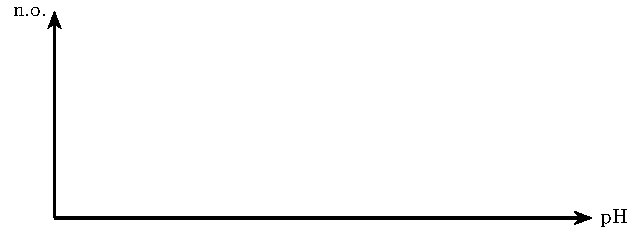
\includegraphics[width=.6\linewidth]{esit_fer-plain}
	% 	}{
	% 		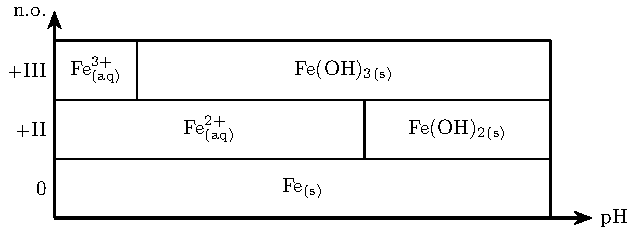
\includegraphics[width=.6\linewidth]{esit_fer}
	% 	}
	% 	\captionsetup{justification=centering}
	% 	\captionof{figure}{Diagramme de situation.}
	% \end{center}
	\begin{enumerate}
		% \bitem{Frontières horizontales}~: ce sont celles des couples
		% $\ce{{Fe}^2+_{\rm(aq)}/Fe}$ et $\ce{{Fe}^3+_{\rm(aq)}/{Fe}^2+_{\rm(aq)}}$.
		% \begin{itemize}
		% 	\item
		% 	      \leftcenters{%
		% 	      $\ce{{Fe}^2+_{\rm(aq)}}/\ce{Fe_{\rm(s)}}$~:
		% 	      }{%
		% 	      \psw{$\ce{Fe_{\rm(s)} = {Fe}^2+_{\rm(aq)} + 2e^-}$}
		% 	      }
		% 	      \vspace{-15pt}
		% 	      \begin{align*}
		% 		      \beforetext{\hspace{2.5cm}$\Ra$}
		% 		      E_1
		% 		                     & =
		% 		      \psw{%
		% 			      E_1^\circ \left( \ce{Fe^2+}/\ce{Fe} \right) +
		% 			      \frac{\num{0.06}}{2} \log \frac{[\ce{Fe^2+}]}{c^\circ}
		% 		      }%
		% 		      \\
		% 		      \beforetext{$[\ce{X}_{\rm(aq)}]\ind{front} = c_t \Ra $}
		% 		      E\ind{1,front} & =
		% 		      \psw{E_1^\circ + \frac{\num{0.06}}{2}\log \frac{c_t}{c^\circ}}
		% 		      \\
		% 		      \beforetext{$c_t = \SI{e-2}{mol.L^{-1}} \Ra$}
		% 		      \makebox[0pt][l]{$\xul{\phantom{E\ind{1,front} = - \SI{0.5}{V}}}$}
		% 		      E\ind{1,front} & =
		% 		      \psw{- \SI{0.5}{V}}
		% 	      \end{align*}
		% 	      \vspace{-15pt}
		% 	\item
		% 	      \leftcenters{%
		% 	      $\ce{{Fe}^3+_{\rm(aq)}}/\ce{{Fe}^2+_{\rm(aq)}}$~:
		% 	      }{%
		% 	      \psw{$\ce{{Fe}^2+_{\rm(aq)} = {Fe}^3+_{\rm(aq)} + e^-}$}
		% 	      }
		% 	      \vspace{-15pt}
		% 	      \psw{%
		% 		      \begin{align*}
		% 			      \beforetext{\hspace{2.5cm}$\Ra$}
		% 			      E_2            & = E_2^\circ \left( \ce{Fe^3+}/\ce{Fe^2+} \right) +
		% 			      \num{0.06} \log \frac{[\ce{Fe^2+}]}{[\ce{Fe^2+}]}
		% 			      \\
		% 			      \beforetext{$[\ce{X}_{\rm(g)}]\ind{front} = c_t \Ra $}
		% 			      \makebox[0pt][l]{$\xul{\phantom{E\ind{2,front} = E_2^\circ = \SI{0.77}{V}}}$}
		% 			      E\ind{2,front} & =
		% 			      E_2^\circ = \SI{0.77}{V}
		% 		      \end{align*}
		% 	      }%
		% \end{itemize}
		% \vspace{-15pt}
		\bitem{Frontières verticales}~:
		\psw{Ce sont les frontières des couples acide-base déterminés plus tôt~:}
		\begin{itemize}
			\item \leftcentersright{%
			      \psw{$\ce{{Fe}^2+_{\rm(aq)}/{Fe(OH)_2}_{\rm(s)}}$\pt{1}~:}
			      }{%
			      \psw{$\ce{{Fe(OH)_2}_{\rm(s)} =
					      {Fe}^2+_{\rm(aq)} + 2 {HO}^-_{\rm(aq)}}$
			      } \pt{1}
			      }{%
			      \psw{$K_{s,2}$}
			      }%
			      \vspace{-15pt}
			      \psw{%
				      \begin{align*}
					      \beforetext{Condition précipité~:}
					      K_{s,2}
					                     & =
					      \frac{[\ce{HO^-}]^2\ind{front}[\ce{Fe^2+}]\ind{front}}{{c^\circ}^3}
					      \pt{1}
					      \\\Lra
					      \pk[s,2]       & =
					      2\pOH\ind{front} - \log c_t/c^\circ
					      \\\Lra
					      \beforetext{$\pOH = \pk[e] - \pH$\pt{1}~:}
					      \Aboxed{
						      \pH\ind{front}
					                     & =
						      \pk[e] - \frac{1}{2}\pk[s,2] - \frac{1}{2} \log c_t/c^\circ
					      }
					      \pt{1}
					      \\\Lra
					      \makebox[0pt][l]{$\xul{\phantom{\xul{\pH\ind{front} = \num{7.5}}}}$}
					      \pH\ind{front} & =
					      \num{7.5} \pt{1}
				      \end{align*}
			      }%
			      \vspace{-15pt}
			\item \leftcentersright{%
			      \psw{$\ce{{Fe}^3+_{\rm(aq)}/{Fe(OH)_3}_{\rm(s)}}$\pt{1}~:}
			      }{%
			      \psw{$\ce{{Fe(OH)_3}_{\rm(s)} =
					      {Fe}^3+_{\rm(aq)} + 3 {HO}^-_{\rm(aq)}}$} \pt{1}
			      }{%
			      \psw{$K_{s,3}$}
			      }%
			      \vspace{-15pt}
			      \psw{%
				      \begin{align*}
					      \beforetext{Condition précipité~:}
					      K_{s,3}
					                     & =
					      \frac{[\ce{HO^-}]^3\ind{front}[\ce{Fe^3+}]\ind{front}}{{c^\circ}^4}
					      \pt{1}
					      \\\Lra
					      \pk[s,3]       & = 3\pOH\ind{front} - \log c_t/c^\circ
					      \\\Lra
					      \beforetext{$\pOH = \pk[e] - \pH$~:}
					      \Aboxed{
						      \pH\ind{front}
					                     & =
						      \pk[e] - \frac{1}{3}\pk[s,3] - \frac{1}{3} \log c_t/c^\circ
					      }
					      \pt{1}
					      \\\Lra
					      \makebox[0pt][l]{$\xul{\phantom{\xul{\pH\ind{front} = \num{2.0}}}}$}
					      \pH\ind{front} & = \num{2.0}
					      \pt{1}
				      \end{align*}
			      }%
		\end{itemize}
		\vspace*{\fill}
		\bitem{Frontières inclinées}~:
		\psw{on étudie la \textbf{pente} des équilibres restants~:}
		\begin{itemize}
			\item \leftcenters{%
			      \psw{$\ce{{Fe(OH)_2}_{\rm(s)}/Fe_{\rm(s)}}$\pt{1}~:}
			      }{%
			      $\psw{\ce{
				      Fe_{\rm(s)} + 2 H_2O_{\rm(l)}
					      =
					      {Fe(OH)_2}_{\rm(s)} + 2 {H}^+_{\rm(aq)} + 2e^-
				      }}$ \pt{1}
			      }%
			      \vspace{-15pt}
			      \psw{%
				      \begin{align*}
					      E\ind{front} & =
					      E^\circ(\ce{{Fe(OH)_2}_{\rm(s)}/Fe_{\rm(s)}}) +
					      \frac{\num{0.06}}{2}
					      \log [\ce{H^+}]^2/{c^\circ}^2
					      \\\Lra
					      E\ind{front} & =
					      E^\circ(\ce{{Fe(OH)_2}_{\rm(s)}/Fe_{\rm(s)}})
					      \xul{\num{-0.06}\pH} \pt{1}
				      \end{align*}
			      }%
			      \vspace{-15pt}
			\item \leftcenters{%
			      \psw{$\ce{{Fe(OH)_3}_{\rm(s)}/{Fe(OH)_2}_{\rm(s)}}$\pt{1}~:}
			      }{%
			      \hspace{20pt}
			      $\psw{\ce{
				      {Fe(OH)_2}_{\rm(s)} + H_2O_{\rm(l)}
					      =
					      {Fe(OH)_3}_{\rm(s)} + {H}^+_{\rm(aq)} + e^-
				      }}$\pt{1}
			      }%
			      \vspace{-15pt}
			      \psw{%
				      \begin{align*}
					      E\ind{front} & =
					      E^\circ(\ce{{Fe(OH)_3}_{\rm(s)}/{Fe(OH)_2}_{\rm(s)}}) +
					      \num{0.06} \log [\ce{H^+}]/c^\circ
					      \\\Lra
					      E\ind{front} & =
					      E^\circ(\ce{{Fe(OH)_3}_{\rm(s)}/{Fe(OH)_2}_{\rm(s)}})
					      \xul{\num{-0.06}\pH} \pt{1}
				      \end{align*}
			      }%
			      \vspace{-15pt}
			\item \leftcenters{%
			      \psw{$\ce{{Fe(OH)_3}_{\rm(s)}/{Fe}^2+_{\rm(aq)}}$\pt{1}~:}
			      }{%
			      $\psw{\ce{
				      {Fe}^2+_{\rm(aq)} + 3 H_2O_{\rm(l)}
					      =
					      {Fe(OH)_3}_{\rm(s)} + 3 {H}^+_{\rm(aq)} + 3e^-
				      }}$ \pt{1}
			      }%
			      \vspace{-15pt}
			      \psw{%
				      \begin{align*}
					      E\ind{front} & =
					      E^\circ(\ce{{Fe(OH)_3}_{\rm(s)}/{Fe}^2+_{\rm(aq)}}) + \num{0.06}
					      \log \frac{[\ce{H^+}]^3}{c_t {c^\circ}^2}
					      \\\Lra
					      E\ind{front} & =
					      E^\circ(\ce{{Fe(OH)_3}_{\rm(s)}/{Fe}^2+_{\rm(aq)}})
					      \xul{\num{-0.18}\pH}\pt{1} - \num{0.06} \log c_t
				      \end{align*}
			      }%
			      \vspace{-15pt}
		\end{itemize}
	\end{enumerate}
	\vspace*{\fill}
	\ifstudent{
		\begin{tikzpicture}[remember picture, overlay]
			\node[anchor=north west, align=left]
			at ([shift={(1.4cm,0)}]current page.north west)
			{\\[5pt]\Large\bfseries Nom~:\\[10pt]\Large\bfseries Prénom~:};
			\node[anchor=north east, align=right]
			at ([shift={(-1.5cm,-17pt)}]current page.north east)
			{\Large\bfseries Note~:\hspace{1cm}/20};
		\end{tikzpicture}
	}
\end{enumerate}
\end{document}
